\section{Tema 2. Equivalencia homotópica}

\subsection{Motivación: Homeomorfismo vs. Homotopía}

Sean $X, Y$ espacios topológicos. Decimos que $X$ e $Y$ son homeomorfos cuando $\exists f \colon X \to Y$ homeomorfismo ($f$ continua, biyectiva, $f^{-1}$ continua).

Equivalentemente: $X \cong Y \iff \exists f \colon X \to Y$ continua, $\exists g \colon Y \to X$ continua, tales que $f \circ g = 1_Y$ y $g \circ f = 1_X$.

\begin{nota}{Notación}{nota_homeomorfismo}
$X \cong Y$ significa que $X$ e $Y$ son homeomorfos. La aplicación identidad en $X$ se denota $1_X \colon X \to X$, $x \mapsto x$ (también se usa $id_X, i_X$).
\end{nota}

En este tema relajaremos las condiciones de la definición de homeomorfismo para llegar a la noción de espacios del mismo tipo de homotopía. Buscamos definir una especie de forma fundamental constante ante contracciones (como ilustra la reducción de un cilindro a una circunferencia o de un cono a un vértice).

\begin{center}
\begin{tikzpicture}[scale=0.8]
  % Cilindro a circunferencia
  \draw (0,2) ellipse (0.8 and 0.3);
  \draw (-0.8,0) -- (-0.8,2);
  \draw (0.8,0) -- (0.8,2);
  \draw (-0.8,0) arc (180:360:0.8 and 0.3);
  \draw[dashed] (0.8,0) arc (0:180:0.8 and 0.3);
  \draw[->] (1.5,1) -- (2.5,1);
  \draw (4,1) ellipse (0.8 and 0.3);
  \node at (0, 2.8) {$X$};
  \node at (4, 1.8) {$Y$};

  % Cono a punto
  \begin{scope}[yshift=-4cm]
      \draw (0,2) -- (-1,0) arc (180:360:1 and 0.3) -- cycle;
      \draw[dashed] (1,0) arc (0:180:1 and 0.3);
      \draw[->] (1.5,1) -- (2.5,1);
      \filldraw (4,1) circle (2pt);
      \node at (0, 2.5) {$\Delta$};
  \end{scope}
\end{tikzpicture}
\end{center}

\subsection{Homotopía entre aplicaciones}

\begin{definicion}{Homotopía entre aplicaciones}{def_homotopia}
Sea $f \colon X \to Y$ aplicación continua. \\
Sea $g \colon X \to Y$ aplicación continua.

Diremos que $f, g$ son homotópicas cuando $\exists F \colon X \times I = [0,1] \to Y$ continua tal que $F_0 = f, F_1 = g$.
\end{definicion}

\begin{nota}{Notación}{nota_homotopia}
Sea $t \in [0,1]$, definimos $F_t \colon X \to Y$ como $x \mapsto F(x,t)$.
\end{nota}

\begin{center}
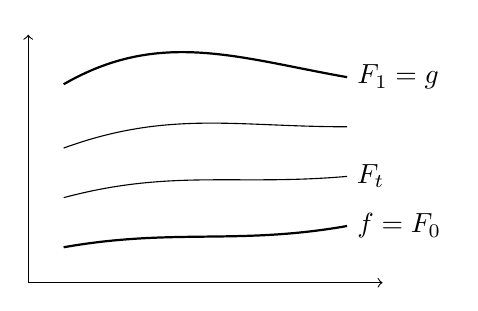
\begin{tikzpicture}[scale=0.9]
    \draw[->] (0,0) -- (0,3.5);
    \draw[->] (0,0) -- (5,0);
    
    \draw[thick] (0.5, 0.5) to[out=10, in=190] (4.5, 0.8) node[right] {$f = F_0$};
    \draw (0.5, 1.2) to[out=15, in=185] (4.5, 1.5) node[right] {$F_t$};
    \draw (0.5, 1.9) to[out=20, in=180] (4.5, 2.2);
    \draw[thick] (0.5, 2.8) to[out=30, in=170] (4.5, 2.9) node[right] {$F_1 = g$};
\end{tikzpicture}
\end{center}

$F$ captura una transformación parametrizada y continua entre $f$ y $g$.

\vspace{0.5cm}
\textbf{Ejemplos:} ¿$f$ y $g$ son homotópicas?

Recordemos que $S^n = \{x \in \mathbb{R}^{n+1} \mid |x| = 1\}$.

\begin{enumerate}
    \item $f \colon S^1 \to S^1, \quad z \mapsto z$ \\
    $g \colon S^1 \to S^1, \quad z \mapsto -z$
    
    $F \colon S^1 \times I \to S^1$ \\
    $(z, t) \mapsto z(\cos(\pi t) + i \sin(\pi t))$. 
    
    Como $F$ es continua y $F_0 = f, F_1 = g$, concluimos que $f$ y $g$ son homotópicas.
    
    \item $f \colon \mathbb{R}^2 \to \mathbb{R}^2, \quad (x,y) \mapsto (x,0)$ \\
    $g \colon \mathbb{R}^2 \to \mathbb{R}^2, \quad (x,y) \mapsto (0,y)$
    
    $F \colon \mathbb{R}^2 \times I \to \mathbb{R}^2$ \\
    $((x,y), t) \mapsto ((1-t)x, ty)$
    
    Por tanto $f$ y $g$ son homotópicas ($f \simeq g$).
\end{enumerate}

\subsubsection{Estructura en $C(X,Y)$}

Llamamos $C(X,Y) = \{f \colon X \to Y \mid f \text{ continua}\}$.

\begin{teorema}{Relación de equivalencia en $C(X,Y)$}{teo_rel_eq}
La homotopía $\simeq$ es una Relación de Equivalencia (R.B.E.) en $C(X,Y)$.
\end{teorema}

\begin{proof}
\begin{enumerate}
    \item \textbf{Reflexiva:} $\forall f \in C(X,Y) \colon f \simeq f$. Basta definir $F \colon X \times I \to Y$ continua mediante $(x,t) \mapsto f(x)$. Evaluando, $F_0 = f$ y $F_1 = f$.
    \item \textbf{Simétrica:} $\forall f,g \in C(X,Y) \colon f \simeq g \implies g \simeq f$.
    Dado que $f \simeq g$, $\exists F \colon X \times I \to Y$ continua tal que $F_0 = f, F_1 = g$.
    Buscamos una $G \colon X \times I \to Y$ continua con $G_0 = g, G_1 = f$.
    Definimos $G(x,t) = F(x, 1-t)$. Es continua por ser composición de funciones continuas y cumple $G_0 = F_1 = g$ y $G_1 = F_0 = f$.
    \item \textbf{Transitiva:} $\forall f,g,h \in C(X,Y) \colon f \simeq g, g \simeq h \implies f \simeq h$.
    Suponemos que $f \simeq^{(1)} g$ y $g \simeq^{(2)} h$. Esto implica que existen $F^{(1)} \colon X \times [0,1] \to Y$ y $F^{(2)} \colon X \times [0,1] \to Y$.
    Necesitamos construir $F \colon X \times I \to Y$ continua con $F_0 = f$ y $F_1 = h$. Definimos:
    \[ F(x,t) = \begin{cases} F^{(1)}(x, 2t) & \forall t \in \left[0, \frac{1}{2}\right] \\ F^{(2)}(x, 2t-1) & \forall t \in \left[\frac{1}{2}, 1\right] \end{cases} \]
    Como $\left(X \times \left[0,\frac{1}{2}\right]\right)$ y $\left(X \times \left[\frac{1}{2}, 1\right]\right)$ son cerrados con restricción continua en la intersección, entonces $F$ es continua. Comprobamos la frontera:
    $F\left(x, \frac{1}{2}\right) = F^{(1)}(x,1) = g(x)$ y $F\left(x, \frac{1}{2}\right) = F^{(2)}(x,0) = g(x)$. Tenemos $F$ bien definida.
    $F_0(x) = F(x,0) = F^{(1)}(x,0) = f(x), \forall x \in X$.
    $F_1(x) = F(x,1) = F^{(2)}(x,1) = h(x), \forall x \in X$.
    Como consecuencia de todo lo anterior, $f \simeq h$.
\end{enumerate}
Por tanto, podremos hablar del espacio cociente $C(X,Y)/\simeq$.
\end{proof}

\begin{teorema}{Composición de homotopías}{teo_comp_homo}
Sean $X \xrightarrow{f_1, f_2} Y \xrightarrow{g_1, g_2} Z$. Si suponemos que $f_1 \simeq f_2$ y $g_1 \simeq g_2$, entonces $g_1 \circ f_1 \simeq g_2 \circ f_2$.
\end{teorema}

\begin{proof}
Tenemos $F \colon X \times I \to Y$ continua con $F_0=f_1, F_1=f_2$.
Tenemos $G \colon Y \times I \to Z$ continua con $G_0=g_1, G_1=g_2$.
Definimos la aplicación $H \colon X \times I \to Z$, $(x,t) \mapsto G(F(x,t), t)$. Evaluamos en los extremos:
\[ H_0(x) = H(x,0) = G(F(x,0), 0) = G(f_1(x), 0) = G_0(f_1(x)) = g_1(f_1(x)), \forall x \in X. \]
\[ H_1(x) = H(x,1) = G(F(x,1), 1) = G(f_2(x), 1) = G_1(f_2(x)) = g_2(f_2(x)), \forall x \in X. \]
Como $H$ es continua, queda probado que $g_1 \circ f_1 \simeq g_2 \circ f_2$.
\end{proof}


\subsection{Equivalencia homotópica entre espacios}

\begin{definicion}{Equivalencia homotópica}{def_eq_homotopica}
Sean $X, Y$ espacios topológicos. Diremos que $X$ e $Y$ son del mismo tipo de homotopía cuando $\exists f \colon X \to Y$ continua y $\exists g \colon Y \to X$ continua tales que $f \circ g \simeq 1_Y$ y $g \circ f \simeq 1_X$. Se denota $X \simeq Y$.
\end{definicion}

\begin{observacion}{Relación con el homeomorfismo}{obs_iso}
$X \cong Y \implies X \simeq Y$.
Tomando $f \colon X \to Y, g \colon Y \to X$ biyecciones donde $g \circ f = 1_X$ y $f \circ g = 1_Y$, se sigue que son trivialmente homotópicas a las identidades ($g \circ f \simeq 1_X$ y $f \circ g \simeq 1_Y$).
\end{observacion}

\textbf{Ejemplos:}
\begin{enumerate}
    \item Sea $X = D(0,1) = \{(x,y) \in \mathbb{R}^2 \mid ||(x,y)|| < 1\}$ y $Y = \{(0,0)\}$.
    Definimos $f \colon X \to Y$, $f = \text{cte}$, es decir, $f(x,y) = (0,0), \forall (x,y) \in X$.
    Definimos $g \colon Y \to X$, $g(0,0) = (0,0)$.
    
    Tenemos que $f \circ g(0,0) = (0,0) \implies f \circ g = 1_Y \implies f \circ g \simeq 1_Y$.
    
    Y también $g \circ f(x,y) = g(0,0) = (0,0), \forall (x,y) \in X \implies g \circ f = c_{(0,0)}$.
    ¿Es $g \circ f = c_{(0,0)} \simeq 1_X$?
    Sea $F \colon X \times I \to X$ continua tal que $F_0 = c_{(0,0)}$ y $F_1 = 1_X$. Podemos definirla como $F((x,y), t) = t \cdot (x,y)$.
    Por tanto, $g \circ f$ es homotópica a la identidad $1_X$, y concluimos que $X \simeq Y$.
    
    \item Sean $X = [-1,1]$ y $Y = \{0\}$.
    Se cumple que $X \not\cong Y$ pero $X \simeq Y$.
    Tomamos $f \colon X \to Y, f = c_0$ y $g \colon Y \to X, g(0) = 0$.
    Claramente $f \circ g = 1_Y$ y $g \circ f = c_0 \simeq 1_X$.
    
    \item Sean $X = S^1 \times [-1,1]$ (cilindro) y $Y = S^1$.
    $f \colon X \to Y, (x,y,z) \mapsto (x,y)$.
    $g \colon Y \to X, (x,y) \mapsto (x,y,0)$.
    
    $f \circ g(x,y) = f(x,y,0) = (x,y) = id_Y, \forall (x,y) \in Y$.
    
    $g \circ f(x,y,z) = g(x,y) = (x,y,0)$. ¿Es homotópica a $1_X, \forall (x,y,z) \in X$?
    Construimos $F \colon X \times I \to X$ (continua por ser polinómica), dada por $F((x,y,z), t) = (x,y, t \cdot z)$. Se verifica que $F_0 = g \circ f$ y $F_1 = 1_X$.
\end{enumerate}
\begin{nota}{Espacios perforados}{nota_agujeros}
$S^2 \setminus \{k \text{ puntos}\} \simeq \bigvee_{j=1}^{k-1} S^1$.
\end{nota}

\subsection{Espacios Contractiles}

\begin{definicion}{Espacio topológico contractil}{def_contractil}
Un espacio topológico $X \neq \emptyset$ es contractil si $\exists x_0 \in X \mid 1_X \simeq c_{x_0}$ (donde $c_{x_0}$ es la aplicación constante $x \mapsto x_0$).
\end{definicion}

\begin{teorema}{Caracterización de espacios contractiles}{teo_contractil}
Son equivalentes las siguientes afirmaciones para un espacio topológico $X \neq \emptyset$:
\begin{enumerate}
    \item[a)] $X$ es contractil.
    \item[b)] $id_X \simeq c_x, \forall x \in X$.
    \item[c)] $\forall f,g \colon T \to X$ continuas $\implies f \simeq g$ (para cualquier espacio topológico $T$).
    \item[d)] $X$ es del mismo tipo de homotopía que un punto.
\end{enumerate}
\end{teorema}

\begin{proof}
$a) \implies b)$: Por hipótesis $\exists x_0 \in X \mid 1_X \simeq c_{x_0}$. Sea $x$ cualquier otro punto de $X$. Sea $c_x$ la aplicación $X \to X, p \mapsto x$.
\[ 1_X \circ c_x \simeq c_{x_0} \circ c_x \implies c_x \simeq c_{x_0} \implies c_x \simeq c_{x_0} \simeq 1_X \]

$b) \implies c)$: Supongamos que $\forall x \in X \colon 1_X \simeq c_x$. Sea $x_0$ cualquier punto de $X \implies 1_X \simeq c_{x_0} \implies 1_X \circ f \simeq c_{x_0} \circ f$.
Para cualesquiera $T \xrightarrow{f,g} X$, se tiene que $f \simeq c_{x_0}$.
Por tanto, $1_X \circ g \simeq c_{x_0} \circ g \implies g \simeq c_{x_0}$ (la composición a una constante envía cualquier $p \mapsto x_0(f(p))=x_0$).
Dado que $f \simeq c_{x_0} \simeq g \implies f \simeq g$.

$c) \implies a)$: Obvio (En particular tomando $T=X$ vemos que $\forall x \in X, 1_X \simeq c_x$).

Las implicaciones $a) \implies d)$ y $d) \implies a)$ quedan como ejercicio directo.
\end{proof}